\documentclass{article}

% if you need to pass options to natbib, use, e.g.:
%     \PassOptionsToPackage{numbers, compress}{natbib}
% before loading neurips_2020

% ready for submission
% \usepackage{neurips_2020}

% to compile a preprint version, e.g., for submission to arXiv, add add the
% [preprint] option:
%     \usepackage[preprint]{neurips_2020}

% to compile a camera-ready version, add the [final] option, e.g.:
%     \usepackage[final]{neurips_2020}

% to avoid loading the natbib package, add option nonatbib:
     \usepackage[nonatbib]{neurips_2020}

\usepackage[utf8]{inputenc} % allow utf-8 input
\usepackage[T1]{fontenc}    % use 8-bit T1 fonts
\usepackage{hyperref}       % hyperlinks
\usepackage{url}            % simple URL typesetting
\usepackage{booktabs}       % professional-quality tables
\usepackage{amsfonts}       % blackboard math symbols
\usepackage{nicefrac}       % compact symbols for 1/2, etc.
\usepackage{microtype}      % microtypography
\usepackage{graphicx}
\usepackage{multicol}
\usepackage{subfig}
\graphicspath{ {./} }
\usepackage{float}
\usepackage{biblatex}
\usepackage{subcaption}
\usepackage[]{graphicx}

\usepackage{physics, amsmath}
\usepackage[margin=1in]{geometry}
\usepackage{bbold}
\DeclareMathOperator*{\E}{\mathbb{E}}
\usepackage{diagbox}
\graphicspath{ {./} }
\usepackage{listings}
\usepackage{xcolor}
\usepackage{bm}
\usepackage{float}
\usepackage{subcaption}
\usepackage{booktabs} 
\usepackage{multirow}
\usepackage{makecell}

\addbibresource{citations.bib}

\usepackage{booktabs}
\usepackage{multirow}
\usepackage{siunitx}



\title{STA 640: Bayesian Non-Parametric Analysis of Heterogenous Treatment Effects.}

% The \author macro works with any number of authors. There are two commands
% used to separate the names and addresses of multiple authors: \And and \AND.
%
% Using \And between authors leaves it to LaTeX to determine where to break the
% lines. Using \AND forces a line break at that point. So, if LaTeX puts 3 of 4
% authors names on the first line, and the last on the second line, try using
% \AND instead of \And before the third author name.

\author{%
  David S.~Hippocampus\thanks{Use footnote for providing further information
    about author (webpage, alternative address)---\emph{not} for acknowledging
    funding agencies.} \\
  Department of Computer Science\\
  Cranberry-Lemon University\\
  Pittsburgh, PA 15213 \\
  \texttt{hippo@cs.cranberry-lemon.edu} \\
  % examples of more authors
  % \And
  % Coauthor \\
  % Affiliation \\
  % Address \\
  % \texttt{email} \\
  % \AND
  % Coauthor \\
  % Affiliation \\
  % Address \\
  % \texttt{email} \\
  % \And
  % Coauthor \\
  % Affiliation \\
  % Address \\
  % \texttt{email} \\
  % \And
  % Coauthor \\
  % Affiliation \\
  % Address \\
  % \texttt{email} \\
}

\begin{document}

\maketitle

\begin{abstract}
  In this paper I propose the use of Ewens-Pitman Attraction (EPA) regression, to perform Bayesian non-parametric regression and clustering for the purpose of identifying treatment effect heterogeneity in randomized experiments. EPA regression is able to simultaneously fit a flexible regression model as well as discover partitions in the sample, the latter of which this work seeks to exploit in finding treatment effect heterogeneity.  
\end{abstract}

\section{Introduction}

One goal of heterogeneous treatment effect (HTE) analysis is to examine if a treatment affects an individual or population subgroup more then others. Identifying such treatment effect heterogeneity is crucial since average or marginal treatment effects may mask the effect of a policy. For example, a subgroup may have a negative treatmeant effect to a medicine whereas the ATE might be positive, it is thus crucial that methods be available to identify such groups. 
\\ \\
The typical approach to HTE analysis is through the use of subgroup analysis. Subgroups are partitions of the covariate space, and are typically pre-specified based on domain knowledge. For example we might specify a males vs females subgroup, and compare difference in treatment effect between the groups. This provides the first motivation for the application of bayesian non-parametric modelling, that such subgroups can be inferred from the data instead of being pre-specified. This is important for several reasons, firstly domain expertise might not be available to specify the subgroups, secondly even with domain expertise a cluster analysis can often times still provide valuable insights into the data, lastly cluster analysis can be useful in finding subgroups in higher dimensions.
\\ \\ 
Besides identifying subgroups, another key part of HTE is that of modelling the Conditional Average Treatment Effect (CATE). In general this can be done several ways, such as with weighting with an IPW estimator. For this work we focus on the outcome modelling approach, where a model is fit to estimate outcomes under all treatment arms. This approach then provides the second motivation for using a bayesian non-parametric approach. Bayesian non-parametrics provides one avenue to specify flexible regression models. In this case, the regression model used is a mixture of linear regression models, where the number of mixture components is dynamic. 
\\ \\
To achieve both aims, a bayesian non-parametric regression model built on the Ewens-Pitman Attraction (EPA) distribution is used (cite chris glynn and dalh). The EPA distribution is a distribution on partitions indexed by a pairwise similarity function (make it nicer). For our application, such similarity is based on the distances between covariates in which we are interested in analysing HTE over. Intuitively, data points with higher similarity in covariates are apriori more likely to be clustered together. EPA regression combines the EPA distribution with a regression sampling model, allowing one to fit a mixture of regressions where data points are allocated to different clusters based on how well a clusters associated parameters can explain a data points outcome - covariate relationship, and its covariate - covariate relationship vis-a-via other points in the cluster. Being a non-parametric clustering model, it also shares the same property as models like the Dirichlet Process mixture model and Pitman Yor mixure model, in that points that are not well explained by existing clusters can start new clusters. In theory, this implies that the model also helps select for the number of clusters, an aspect that is often left as a hyperparameter in most clustering algorithms.
\\ \\ 
\section{Related Work}

The EPA distribution is introduced in \cite{dahl2017random} as a distribution over partitions with pairwise similarity information. Here the author demonstrates its use in unsupervised non-parametric clustering models as well as in a non-parametric regression setting. EPA regression is applied to the model of homeless rates across different spatial locations in \cite{glynn2021inflection}, here the authors focus is on analysing the regression surface, to find inflection points relating covariates to homeless rates. Their use of EPA regression is motivated by the hypothesis that these spatial locations are likely to be similar to each other.  A key difference however is that the work does not aim to find a causal effect.

Lastly, the work of causal clustering in \ref{kim2020causal}, also seeks to discover latent subgroups in the data with heterogenous treatment effects. The approach however is different. With causal clustering the author first uses an outocme model to estimate the vector of potential outcomes. These estimated potential outcomes are passed into a clustering algorithm like K-means or hierarchical clustering in order to find clusters of data points in the potential outcome space. These clusters, if they exist are likely to have differing levels treatment effect. Our work is different in that we exploit the EPA regression model's ability to model and cluster jointly, bypassing the need to fit outcome and clustering model separately. 

\section{Model}
\label{sec:Model}
\paragraph{Causal Estimand and Setup} We consider either an observational or randomized control trial consisting of $n$ iid samples. Each sample $i$ is an tuple $(Y_i, D_i, X_i, Z_i)$. Where $Y_i$ is the treatment outcome, $D_i$ is the assigned treatment, $X_i$ are covariates and $Z_i$ are variables we seek to perform HTE analysis over. Note that it is generally the case that $Z_i = X_i$ or $Z_i$ is a subset of the variables in $X_i$. We further consider the case of a continuous outcome, that is $Y_i$ is continuous and a binary treatment, that is $D_i \in {0,1}$. $X_i$ and $Z_i$ are vectors $d$ and $p$ dimenionsal vectors and can be of mixed continuous and categoricals elements. For treatment effect identification with have the following assumptions.
\begin{itemize}
    \item SUTVA: ...
    \item Positivity ... 
    \item No unmeasured confounding ...
\end{itemize}
For randomized control trials, assumption A3 is automatically fulfilled due to the randomized nature of treatment assignment $D_i$. For observational studies, A3 implies that any confounders of $D_i$ and $Y_i$ are observed in the set $X_i$. 
\\ \\
The causal quantity of interest is the conditional average treatment effect (CATE) given by:
$$CATE(X) = E[Y(1)-Y(0)|X]$$ 
\\ 
Under the assumptions, CATE can be identified as:
$$E[Y(1)-Y(0)|X] = E[Y|D=1] - E[Y|D=0]$$ 
\\ 
Thus the modelling approach is to specify models for $E[Y|D=1]$ and $E[Y|D=0]$. For this work, we take the S-learner approach, where a single model $Y=f(D,X)$ is specified and we take $f(1,X) = E[Y|D=1]$ and $f(0,X) = E[Y|D=0]$. The estimator for CATE is then:
$$\widehat{CATE(X)} = f(1,X) - f(0,X)$$ 
where $f$ is the EPA regression model.

\paragraph{EPA Distribution}

The EPA distribution is a distribution over partitions indexed by a pairwise similarity function, a mass parameter $\alpha$ and a discount parameter $\delta$. That is, suppose we have points $X_1,...,X_n$ and a similarity function $\lambda(X_i,X_j)$. Denote $\pi_t$ as partition of the dataset of the first $t$ data points. The distribution is then given by:

\begin{equation}
\label{eqn:EPA Distribution}
P(\pi_n| \alpha, \delta, \lambda, \sigma) = \prod_{t=1}^n P_t(\alpha, \sigma, \lambda, \pi(\sigma_1,...,\sigma_{t-1}))
\end{equation}

Where each $P_(t)$ is given by.

\begin{equation}
\begin{align*}
    P_t(\alpha, \sigma, \lambda, \pi(\sigma_1,...,\sigma_{t-1})) &= P(\sigma_t \in S|\alpha, \delta,\lambda, \pi(\delta_1,...,\delta_{t-1}) \\
    &=\begin{cases}
    \frac{t-1-\delta q_{t-1}}{\alpha + t-1}\frac{\sum_{\sigma_s \in S}\lambda(\sigma_t,\sigma_s)}{\sum_{s=1}^{t-1}\lambda(\sigma_t,\sigma_s)}, & \text{if } S \in \pi(\sigma_1,...,\sigma_{t-1}) \\
     \frac{\alpha + \delta q_{t-1}}{\alpha+t-1}, & \text{if \emph{S} in a new subset}
    \end{cases} 
\end{align*}
\end{equation}

Where $q_{t-1}$ is the number of clusters in the $t-1$ partition. $\sigma_i$ refers to the ordering of the data, which is not necessarily the same as the order in the dataset. That is the model is not exchangeable, this is an important fact that has to be accounted for when doing gibbs sampling. Looking at the equation, we can see that the EPA distribution allocates items sequentially, with probabilities proportion to the total similarity between an item and items currently allocated in a cluster, at the same time, there is also a chance that the distribution allocates the item to a new cluster, which is more likely if the similarities to existing clusters are small.
\\ \\
The similarity function we use is the exponential similarity function, given by:
\begin{equation}
    \lambda(X_{\lambda_s}, X_{\lambda_t}) = \text{exp}\{-\tau \lVert X_{\lambda_s} - X_{\lambda_t} \rVert  \}
\end{equation}
Which is similar to the popular radial basis function but paramatized by a precision term $\tau$ instead of the usual $\frac{1}{2\sigma^2}$. We take $\tau$ to be a hyperparameter, but it can generally be taken as a parameter to be inferred as well.
    
\paragraph{Outcome Model}
The modelling approach is a non-parametric regression model for the observations $Y_i$ given the treatment assignments $D_i$ and covariates (or possibly confounders) $X_i$. To this end we specify the regression likelihood. Each observation $Y_i$ is modelled as a linear function of $D_i$, $X_i$ and possible interaction effects. That is:
\begin{equation}
    Y_i = \phi_{0i} + \phi_{1i}D_i + \phi_{2i}X_i + \epsilon
\label{reg_ll}
\end{equation}
Where $\epsilon \sim N(0,\sigma^2)$. Letting $\phi_i$ be the regression coefficient vector for the $i^{th}$ data point, $\phi_i = (\phi_{0i}, \phi_{1i}, \phi_{2i})$, we have that $\phi_i$ is taken as the cluster specific parameter vector, that is, where $Z_i$ is the cluster index of the $i^{th}$ data point:
\begin{equation}
    \phi_i = \sum_{k=1}^{q_n} \tilde{\phi_k} \mathbb{1}_{\{Z_i=k}\}
\end{equation}
Each $\tilde{\phi_k}$ is drawn independently from a multivariate normal prior, where the prior mean and covariance serve as hyperparameters.

\paragraph{Model Inference} 
Inference proceeds by way of a Gibbs - Sampler over the parameters $\pi$, $\phi$, $\alpha$, $\delta$ and $\beta$. For $\pi$ the Gibbs sampler iterates over each data point, proposing for each data point a possible move to other existing clusters, or starting a new cluster. This is given by :
\begin{equation}
    P(i \in S_j^{-i} |.) \propto P(\pi_n^{i \rightarrow j} | \alpha, \delta, \lambda, \sigma)P(Y_i | \tilde{\phi_j})  \quad \text{,for } j=0,1,...,q_n
\end{equation}
Where $S_j^{-i}$ refers to $j^{th}$ subset but without point $i$ and $\pi_n^{i \rightarrow j}$ is the partition obtained by moving point $i$ to cluster $S_j^{-i}$.
\\ \\
Inference of $\tilde{\phi_k}$ is similar to inference in a hierarchical model with no pooling. That is, each $\tilde{\phi_k}$ is updated only by points allocated to its cluster $k$. With our normal likelihood and normal prior over $\tilde{\phi_k}$ in \ref{reg_ll}, the updates are conditionally conjugate given the partition. That is:
\begin{equation}
    \tilde{\phi}_k | \pi_n, \alpha, \delta, \beta, \sigma \sim N(\tilde{\mu}_k, \tilde{\Sigma}_k). 
\end{equation}
Where $\tilde{\mu}_k = $ and $\tilde{\Sigma}_k=$.
\\ \\ 
We refer readers to \cite{dahl2017random} for details on sampling $\alpha$, $\beta$ and $\sigma$, generally these are sampled using a metropolis in gibbs scheme, where we take a metropolis-hasting step to sample these parameters. For proposal distributions, we generally use random walks. Note that for for $\sigma$ we use a uniform prior and a uniform proposal. 
\section{Data}
We experiment with two datasets. A simulated dataset as well as the National Supported Work Demonstration (NSW) dataset.

\paragraph{Simulated Dataset} This dataset consists of xx simulated data points from 3 latent regression functions. Index these latent regression functions by 1,2,3 respectively. We firstly generate 1D covariates $X_k$ from Gaussian distributions centered at x x and x with standard deviations x x and x. For each cluster $k$ x points are generated. Then we specify 3 regression functions.

\begin{equation}
\label{eqn:latent_reg1}
Y_{i1} = 0.3 * D_{i1} + 0.5*X_{i1} + 0.6*X_{i1}*D_{i1} + \sigma_1
\end{equation}
\begin{equation}
\label{eqn:latent_reg1}
Y_{i2} = 0.3 * D_{i2} + 0.5*X_{i2} + 0.6*X_{i2}*D_{i2} + \sigma_2
\end{equation}
\begin{equation}
\label{eqn:latent_reg1}
Y_{i3} = 0.3 * D_{i3} + 0.5*X_{i3} + 0.6*X_{i3}*D_{i3} + \sigma_3
\end{equation}

Each treated $D_ik$ is generated at random with $P(D_ik) = 0.5$, meaning that treatment in this simulated dataset is randomly assigned. Lastly the values of $Y_{ik}$ are generated based one generated $X_{ik}$ and the randomly assigned $D_{ik}$. A plot of the dataset can be seen in figure \ref{fig:sim_data_info}, which shows histograms and scatter plots of the true treatment effects, the scatter plots of the treatment effects against the covariate $X$, and of histogram and scatter plots of the observed data against the covariate $X$. We can see from these plots the presence of treatment effect heterogeneity as a function of the covariate $X$. 

\paragraph{National Supported Work Demonstration (NSW) Data} The National Supported Work Demonstration job training was a experimental program ran in the 1970s by Manpower Demonstration Research Corp (MRDC). The program involved giving participants temporary employment which was designed to help those lacking basic job skills move into the labor market by giving them work experience. The dataset consists of 405 individuals along with x covariates consisting of demographic information, educational background as well as income levels prior to the program. The outcome we measure is the income level post the program. 
\\ \\ 
For the NSW data, we take a further subset of xx individuals who are employed at the end of the program period (whether they were treated or not), this is for computational reasons, with the 0 data points affecting the gaussian likelihood. It is important to note however that effects estimated here are thus not representative of the population that the NSW data sets out to measure the policies effectiveness over.


\section{Modelling and Results}
In this section we discuss the modelling details for each dataset as well as the results. 

\subsection{Modelling Parameters}
\paragraph{Simulated Data}
For the simulated dataset, we fit the EPA regression model with a Gaussian likelihood and interaction effects. That is:
$$Y_i = \beta_{0k} + \beta_{1k}D_i + \beta_{2k}X_i + \beta_{3k}X_iD_i$$ We fixed the regression error $\sigma$ as 1. The prior on $\alpha$ is a $Ga(1,10)$ distribution, and the prior on $\beta$ is a mixture of a point mass at 0 and a $\beta(1,1)$ distribution, with each mixture component having an identical weight of 0.5. The prior on $\phi$ is a multivariate normal with 0 mean and an identity matrix as the covariance.  For this model we generated a total of 10000 gibbs sample, with 5000 being discarded as burn-in. 

\paragraph{NSW Data} For the NSW data, we fit EPA regression model with a Gaussian likelihood but without interaction effects. That is:
$$Y_i = \beta_{0k} + \beta_{1k}D_i + \beta_{2k}X_i$$ where $X_i$ is a vector of covariates. We remove interaction effects as we find it results in too many parameters, leading to poor fit of the model. Further we transform the outcome $Y$ by analysing in 1000s that is dividing $Y$ by 1000. This is to avoid having to set large prior values for $\phi$ parameters. Since the treatment is randomized, we first take a simple difference in mean between treatment and control to estimate the sample average treatment effect, this gives a value of \$1340.84.
\\ \\
Prior distributions on $\alpha$ and $\beta$ is identical to that used for the model on the simulated data. For $\phi$ we use a zero-mean Gaussian distribution, with a diagonal covariance matrix. This covariance has 1s in all diagonal elements except for the intercept term and the treatment treat, for which the prior variance are 3 and 2 respectively. For this model we generated a total of 15000 gibbs sample, with 5000 being discarded as burn-in. 

\subsection{Simulated Dataset Results} 
For the simulated data, we know the underlying latent clusters and associated regression function for each data point. We thus benchmark the model based how close the model estimated clustering is to the ground truth clusters and treatment effects.
\\ \\
Firstly, we conduct several regression diagnostics by looking at plots of $Y_{obs}$ vs $\hat{Y}$, and the histogram of residuals and plots of residuals vs $Y_{obs}$, these are shown in figure \ref{fig:sim_diag_plots}. We see no major issues, with the residuals having a symmetrical distribution around 0, and the residuals being homoskedastic over the range of $Y$.
\paragraph{Obtaining Clusters} One issue to note is that our model outputs Monte Carlo samples of possible partitions. There is thus a need to post-process the set of samples to one coherent cluster assignment. For this we take the approach of \ref{medvedovic2004bayesian} which applies hierarchical clustering to the posterior similarity matrix. We plot the posterior similarity matrix for the simulated data in figure \ref{fig:sim_post_mat}, showing the clear presence of 3 clusters. 
\\ \\
Using this approach, we find that (unsurprisingly) a 3 cluster solution is the most reasonable, that is 4,5 and 6 cluster solutions produced singleton clusters. Further looking at the posterior partition samples, we found that the average number of unique partitions is also 3. Figure \ref{fig:sim_scatter_plots} plots the obtained cluster solutions over the $Y^{obs}$ vs $X$ scatter plot. We see that the results almost perfectly match the true latent clustering, indicating the model is able to detect the latent clusters corresponding to the heterogeneous treatment effects. 

\paragraph{Predicting Potential Outcomes} We choose not to analyse parameters associated to each cluster due to label switching. Instead we analyse each cluster by looking at the mean predicted treatment effect for that cluster. For this we use the Monte Carlo samples to estimate for each individual $i$ the potential outcomes $Y_i(1)$ and $Y_i(0)$ as $\hat{f}(1,X)$ and $\hat{f}(0,X)$ respectively. Figure \ref{fig:sim_scatter_plots} plots the estimated ITEs against the covariates $X$, as well as the estimates of potential outcome under one treatment arm to the other. We can see here that the treatment effect has a strong linear effect with $X$, similar to that of thettrue effects. Note that these are mean estimates for each ITE, explaining why the scatter is linear in nature (for each cluster). Figure \ref{fig:sim_histo} plots histograms of mean $ITE$ separated by clusters, table \ref{tab:simulated_ITEs} shows the mean of ITEs per cluster compared to that of the true mean ITE, we see that generally the predicted cluster means of ITEs align with that of the true means, however the values of the predicted are consistently smaller, this is likely due the shrinkage effect of the bayesian model, as well as the relatively tight standard normal prior.

\subsection{NSW Dataset Results} 
Proceeding with the same cluster aggregation approach as with the simulated data, we find 5 clusters with in the dataset. We intially specified the hierarchical clustering procedure with 8 clusters, but found the 3 out of the 8 had insignificant support, hence we do not anaylse the outcomes for the 10 points contained within those clusters. Figure \ref{fig:nsw_post_mat} plots the posterior similarity matrix. 
\\ \\
Figure \ref{fig:nsw_diag_plots} plots the same diagnostics as those done for the simulated data, we can see an overall poorer fit of the model for the NSW data. We can see that generally, the predicted $Y$ match the observed $Y$, with residuals being centered around 0, we do however observe a heavier left tail, and a larger variance of residuals close to when $Y_{obs}$ is near 0. We believe this is due to issue with using the Gaussian likelihood for data which is theoretically bounded below by 0.
\\ \\
Figure \ref{fig:nsw_scatter_plots} shows a scatter plot of estimated treatment effects in one arm against the other, overlaid with colors of clustering indices, here deviation from the 45\% line indicates size of the treatment effect. Similar information is shown in figure \ref{fig:nsw_histo}, with shows histograms of mean ITEs for each cluster, and table \ref{tab:nsw_ate_results} shows the point estimates along with the standard deviation. We see the presence of some heterogeneity in treatment effects, with most clusters having mean effect around 0, and several having larger treament effects, such as a cluster of 32 points having ATE of \$660 dollars. Importantly we see that these effects are well below the SATE of \$1340.84. This could imply a degree of over-shrinkage by the Bayesian model, or a strong presence of HTEs. 
\\ \\
To look at possible drivers behind the HTE, we look at the distribution of covariates $X$ across the different clusters. This is shown in figure x.  


\section{Conclusion}
In this work, we have explored the use of the Log Gaussian Cox Process to build a spatio-temporal Model of crime rates in Chicago. Two extensions, an Intrinsic Coregionalization Model for modelling multi-outputs and Kronecker Covariance, for scaling the model to larger datasets, were explored. The latter enabled us to fit the model various models within a reasonable amount of time, and with a reasonable amount of compute, whereas the former out-performed models where each crime type were fitted independently. Further, based on our benchmarking, we saw that the ICM extension was essential in building a predictive model which outperformed baseline's consistently. Overall, we have demonstrated that these Gaussian process models are both accurate, and also have the potential to scale, thus demonstrating the potential of their use in modelling the complex crime occurrence data. 




\appendix

\section{Simulated Data Plots}
This section contains plots related to the simulated the simulated dataset.
\begin{figure}[h]
  \centering
  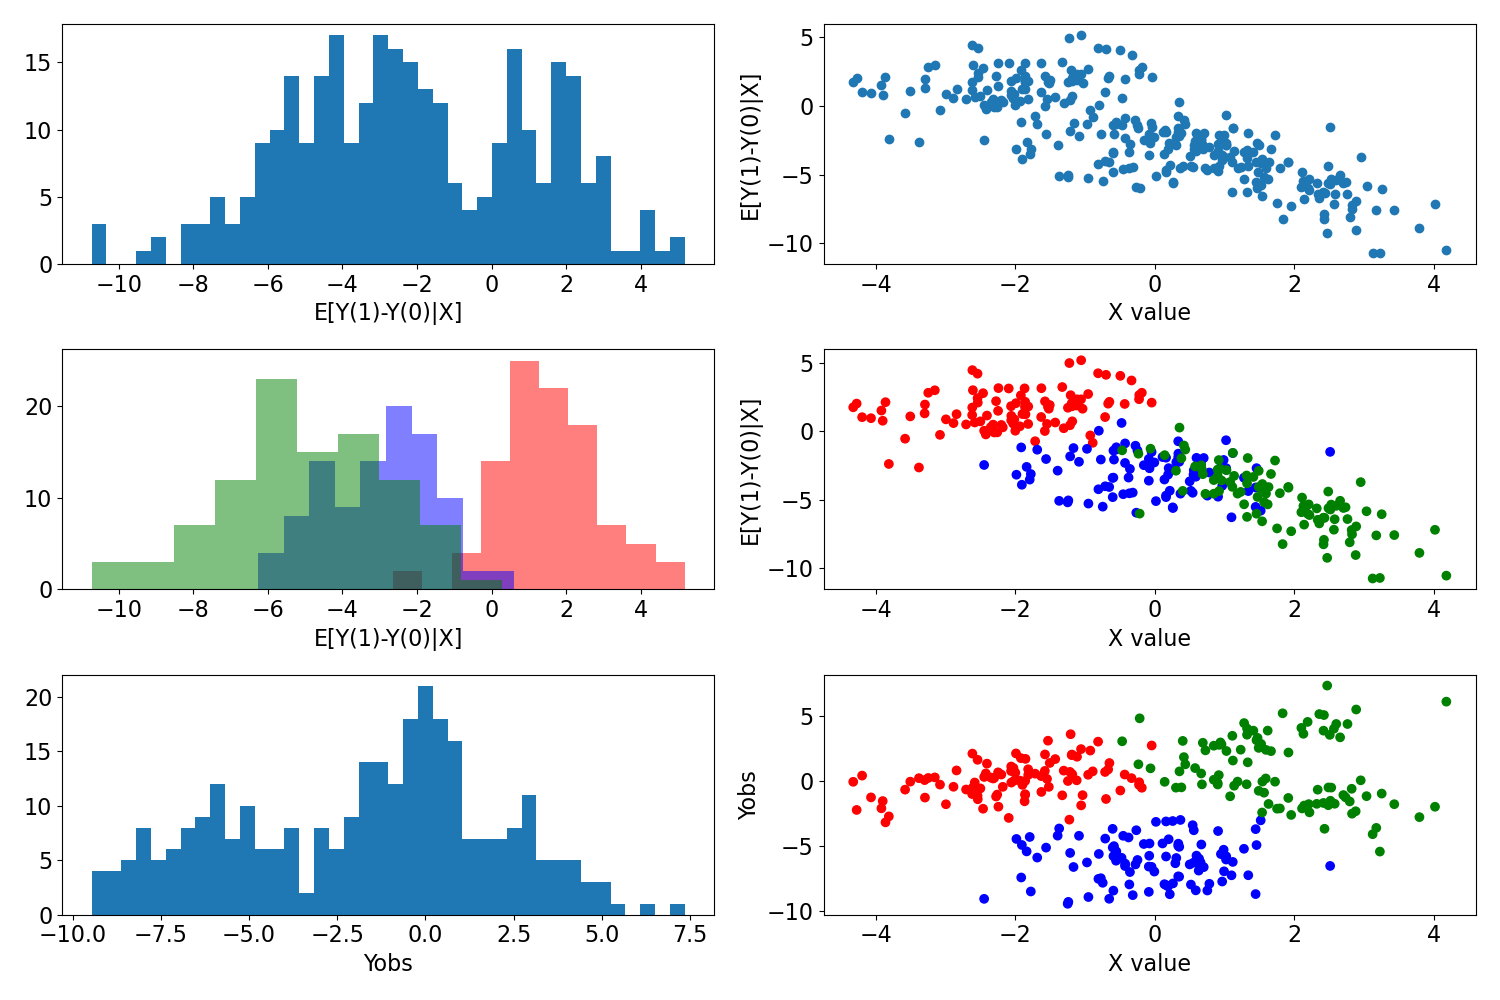
\includegraphics[width=1\textwidth]{Plots/simulated_data_info.png}
  \caption{Various plots of the simulated dataset. Top Row: Histogram of true ITES and scatter plots of true ITEs vs X. Midlde Row: iHstogram of true ITES and scatter plots of true ITEs colored by true latent cluster index. Bottom Row: Histogram of observed outcomes and scatter plots of observed outcomes colored by true latent cluster index.}
  \label{fig:sim_data_info}
\end{figure}

\section{Simulated Data Results}
This section contains plots related to the model outputs from analysising the simulated dataset.

\begin{figure}[h]
  \centering
  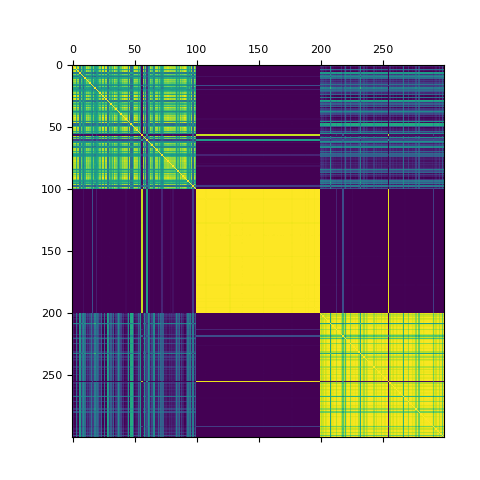
\includegraphics[width=0.8\textwidth]{Plots/Simulated Posterior Similarity Matrix.png}
  \caption{Posterior similarity matrix inferred from simulated data}
  \label{fig:sim_post_mat}
\end{figure}

\begin{figure}[h]
  \centering
  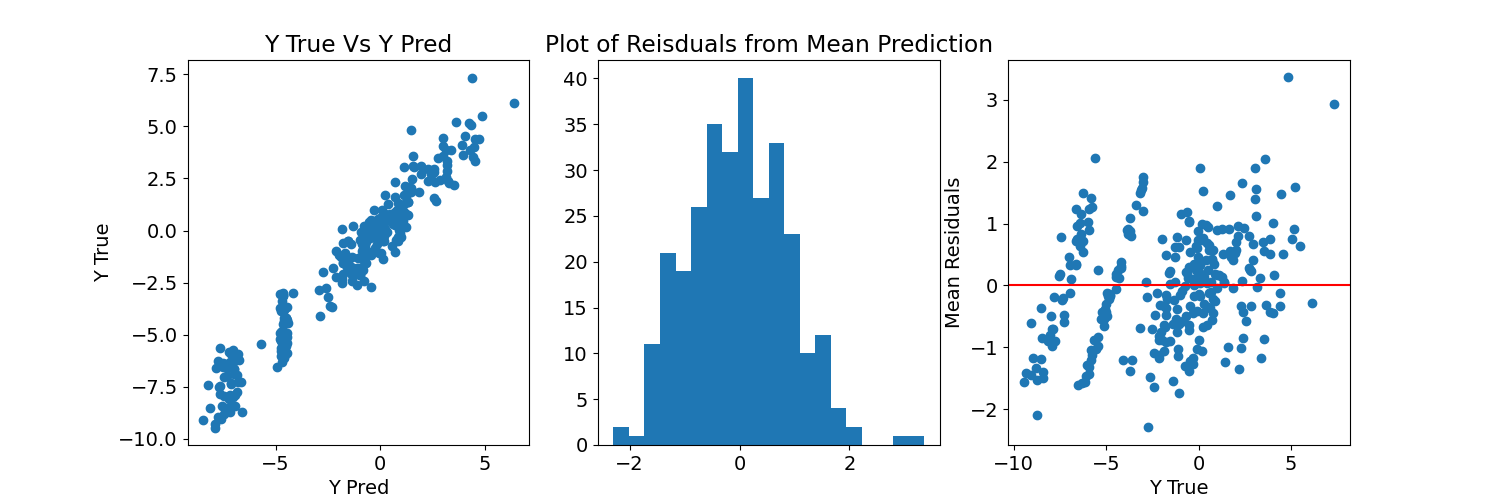
\includegraphics[width=1\textwidth]{Plots/simuated_diagnostics.png}
  \caption{Various regression diagnostic plots for model on simulated data. Left: Y True vs Y Predicted. Middle: Histogram of mean residuals. Right: Scatter plot of mean residual vs Y True}
  \label{fig:sim_diag_plots}
\end{figure}

\begin{figure}[h]
  \centering
  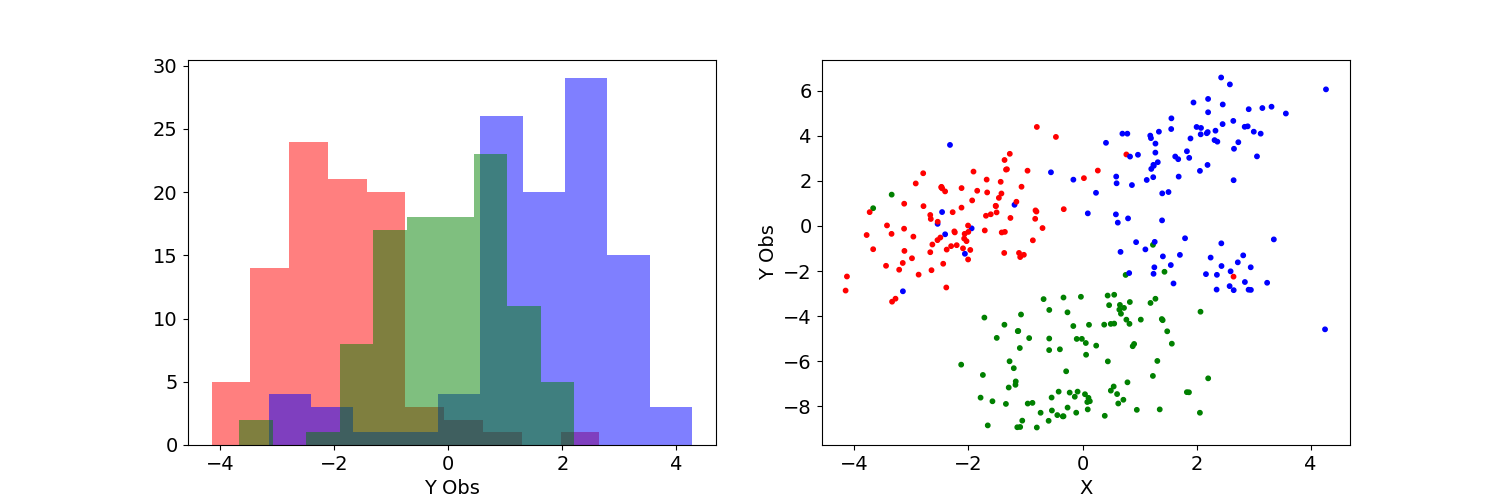
\includegraphics[width=1\textwidth]{Plots/simulated_cluster_scatter.png}
  \caption{Left: Histogram of Y Obs colored by posterior cluster groupings. Right: Scatter plot of Y Obs against X colored by posterior cluster groupings.}
  \label{fig:sim_scatter_plots}
\end{figure}

\begin{figure}[h]
  \centering
  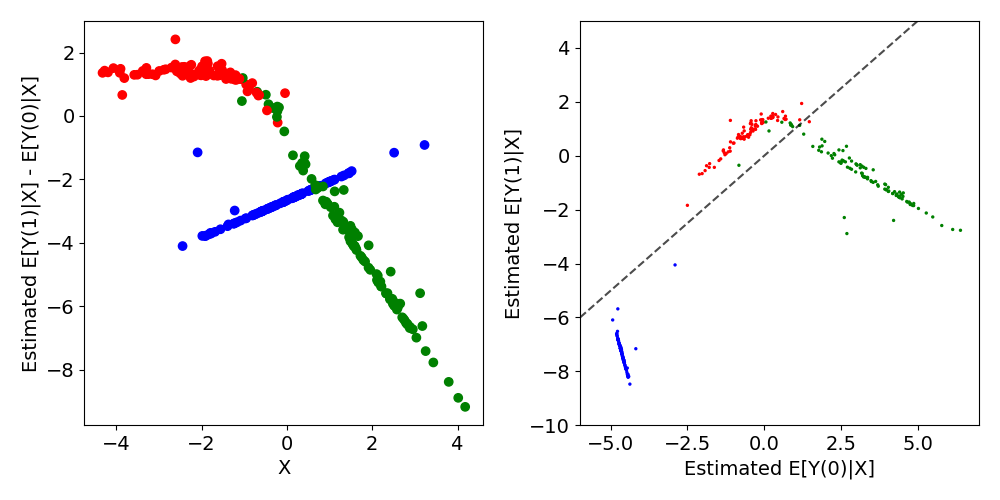
\includegraphics[width=1\textwidth]{Plots/Simulated_output_scatted.png}
  \caption{Scatter plots of estimated individual treatment effects for model on simulated data. Left: Estimated individual treatment effect against X, colored by estimated cluster index. Right: Plot of $\hat{E}[Y(1)]$ against $\hat{E}[Y(0)]$}
  \label{fig:sim_scatter_plots}
\end{figure}

\begin{table}[h]
\centering
\begin{tabular}{cc}
\hline
True Mean ITE & Predicted Mean ITEs \\
\hline
1.56 & 1.30 \\
-3.03 & -2.66 \\
-4.98 & -3.97 \\
\hline
\end{tabular}
\caption{True and predicted mean ITEs}
\label{tab:simulated_ITEs}
\end{table}



\begin{figure}[h]
  \centering
  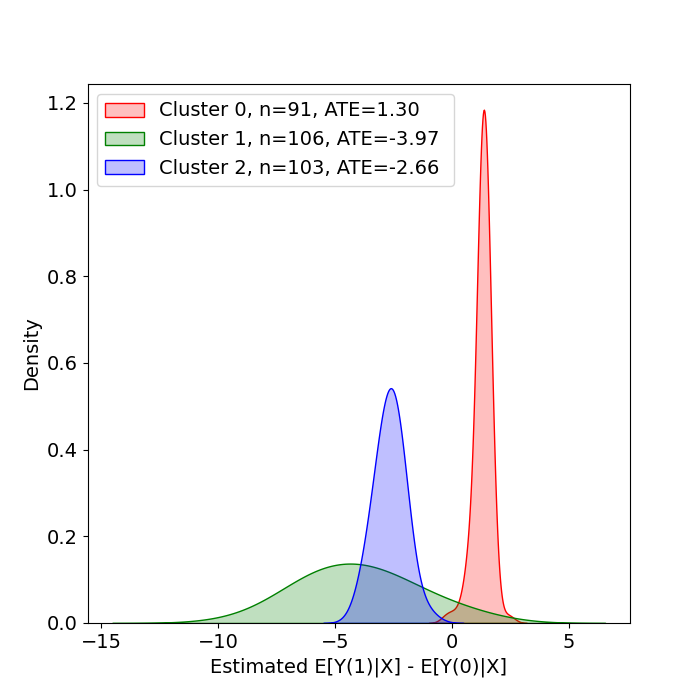
\includegraphics[width=0.8\textwidth]{Plots/Simulated_output_histogram.png}
  \caption{KDE plots of estimated ITEs by cluster indexes. For model on simulated data}
  \label{fig:sim_histo}
\end{figure}


\section{NSW Data Results}
This section contains plots related to the model outputs from analysising the NSW dataset.
\begin{figure}[h]
  \centering
  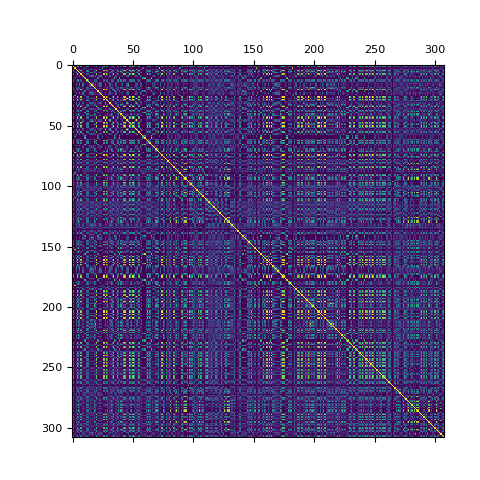
\includegraphics[width=0.8\textwidth]{Plots/NSW Posterior Similarity Matrix.png}
  \caption{Posterior similarity matrix inferred from NSW data}
  \label{fig:nsw_post_mat}
\end{figure}

\begin{figure}[h]
  \centering
  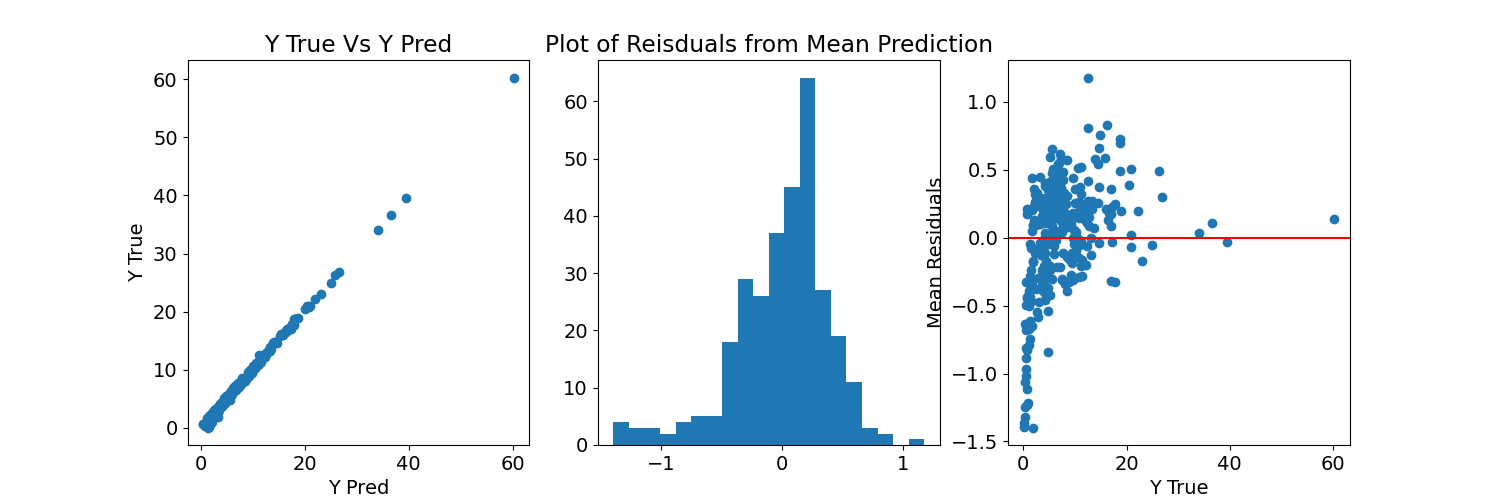
\includegraphics[width=1\textwidth]{Plots/NSW_diagnostics.png}
  \caption{Various regression diagnostic plots for model on NSW data. Left: Y True vs Y Predicted. Middle: Histogram of mean residuals. Right: Scatter plot of mean residual vs Y True}
  \label{fig:nsw_diag_plots}
\end{figure}

\begin{figure}[h]
  \centering
  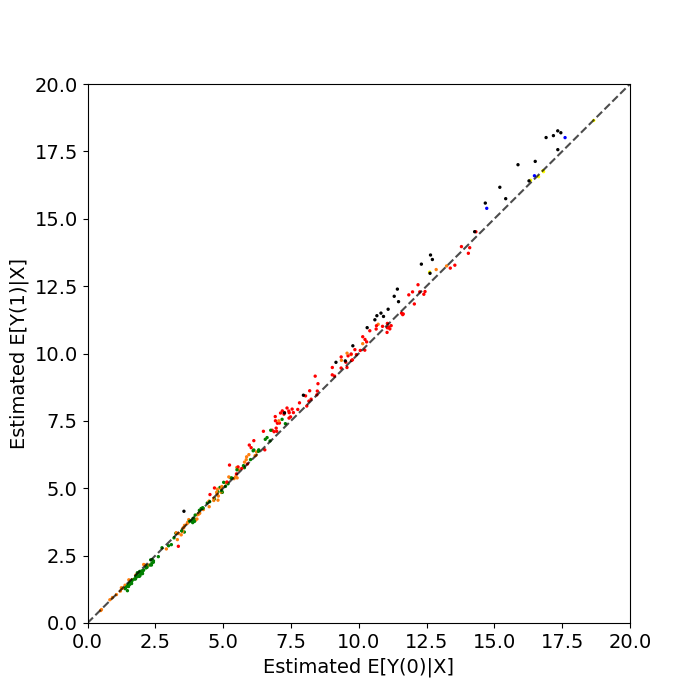
\includegraphics[width=0.8\textwidth]{Plots/NSW_output_scatted.png}
  \caption{Scatter plots of estimated individual treatment effects for model on NSW data. Estimated individual treatment effect against X, colored by estimated cluster index}
  \label{fig:nsw_scatter_plots}
\end{figure}

\begin{figure}[h]
  \centering
  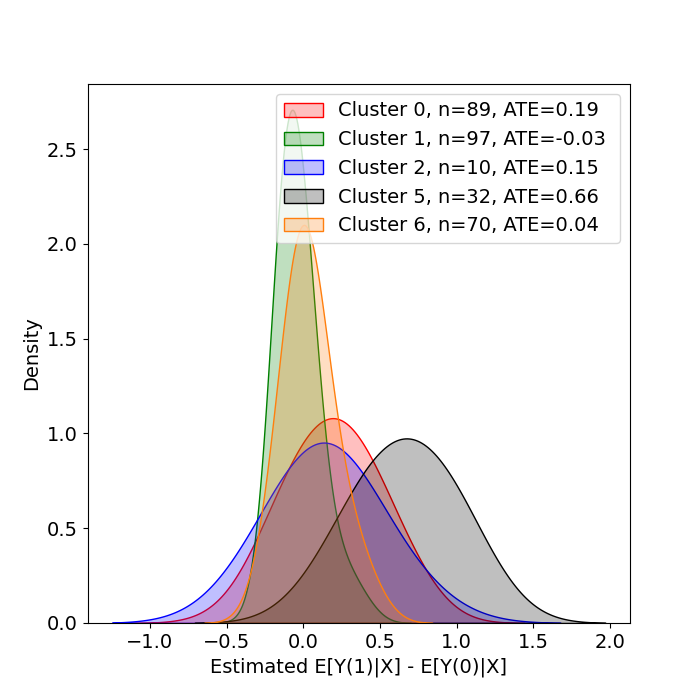
\includegraphics[width=0.8\textwidth]{Plots/NSW_output_histogram.png}
  \caption{KDE plots of estimated ITEs by cluster indexes. For model on NSW data}
  \label{fig:nsw_histo}
\end{figure}

\begin{table}[H]
\centering
\label{tab:cluster_ate}
\begin{tabular}{c|c c}
\hline
\textbf{Estimated Cluster} & \textbf{Cluster ATE} & \textbf{SD Cluster ATE} \\ \hline
0 & 193.17 & 275.42 \\
1 & -34.14 & 126.85 \\
2 & 148.67 & 252.92 \\
5 & 661.50 & 274.61 \\
6 & 39.76 & 152.22 \\
\hline
\end{tabular}
\caption{Cluster ATE estimates and standard deviations for estimated clusters}
\label{tab:nsw_ate_results}
\end{table}

\begin{table}[H]
\centering
\label{tab:clusters}
\begin{tabular}{c|c|c|c|c|c}
\hline
\textbf{Estimated Clusters} & N &\textbf{black} & \textbf{hisp} & \textbf{marr} & \textbf{nodegree} \\ \hline
0 & 89 & 0.808989 & 0.067416 & 0.146067 & 0.730337 \\
1 & 97 & 0.783505 & 0.134021 & 0.195876 & 0.845361 \\
2 & 10 & 0.800000 & 0.200000 & 0.200000 & 0.700000 \\
5 & 32 & 0.781250 & 0.062500 & 0.125000 & 0.812500 \\
6 & 70 & 0.771429 & 0.142857 & 0.185714 & 0.714286 \\
\hline
All & 298 & 0.788591 & 0.110738 & 0.171141 & 0.771812  \\
\hline
\end{tabular}
\caption{Proportion of black, hisp, marr, and nodegree for each cluster}
\label{tab:nsw_cluster_covar_discrete}
\end{table}




\printbibliography

\end{document}
